\PassOptionsToPackage{unicode=true}{hyperref} % options for packages loaded elsewhere
\PassOptionsToPackage{hyphens}{url}
%
\documentclass[]{book}
\usepackage{lmodern}
\usepackage{amssymb,amsmath}
\usepackage{ifxetex,ifluatex}
\usepackage{fixltx2e} % provides \textsubscript
\ifnum 0\ifxetex 1\fi\ifluatex 1\fi=0 % if pdftex
  \usepackage[T1]{fontenc}
  \usepackage[utf8]{inputenc}
  \usepackage{textcomp} % provides euro and other symbols
\else % if luatex or xelatex
  \usepackage{unicode-math}
  \defaultfontfeatures{Ligatures=TeX,Scale=MatchLowercase}
\fi
% use upquote if available, for straight quotes in verbatim environments
\IfFileExists{upquote.sty}{\usepackage{upquote}}{}
% use microtype if available
\IfFileExists{microtype.sty}{%
\usepackage[]{microtype}
\UseMicrotypeSet[protrusion]{basicmath} % disable protrusion for tt fonts
}{}
\IfFileExists{parskip.sty}{%
\usepackage{parskip}
}{% else
\setlength{\parindent}{0pt}
\setlength{\parskip}{6pt plus 2pt minus 1pt}
}
\usepackage{hyperref}
\hypersetup{
            pdftitle={Usando Biologia de Sistemas para entender a Imunossenescência},
            pdfauthor={Fernando Marcon Passos},
            pdfborder={0 0 0},
            breaklinks=true}
\urlstyle{same}  % don't use monospace font for urls
\usepackage{color}
\usepackage{fancyvrb}
\newcommand{\VerbBar}{|}
\newcommand{\VERB}{\Verb[commandchars=\\\{\}]}
\DefineVerbatimEnvironment{Highlighting}{Verbatim}{commandchars=\\\{\}}
% Add ',fontsize=\small' for more characters per line
\usepackage{framed}
\definecolor{shadecolor}{RGB}{248,248,248}
\newenvironment{Shaded}{\begin{snugshade}}{\end{snugshade}}
\newcommand{\AlertTok}[1]{\textcolor[rgb]{0.94,0.16,0.16}{#1}}
\newcommand{\AnnotationTok}[1]{\textcolor[rgb]{0.56,0.35,0.01}{\textbf{\textit{#1}}}}
\newcommand{\AttributeTok}[1]{\textcolor[rgb]{0.77,0.63,0.00}{#1}}
\newcommand{\BaseNTok}[1]{\textcolor[rgb]{0.00,0.00,0.81}{#1}}
\newcommand{\BuiltInTok}[1]{#1}
\newcommand{\CharTok}[1]{\textcolor[rgb]{0.31,0.60,0.02}{#1}}
\newcommand{\CommentTok}[1]{\textcolor[rgb]{0.56,0.35,0.01}{\textit{#1}}}
\newcommand{\CommentVarTok}[1]{\textcolor[rgb]{0.56,0.35,0.01}{\textbf{\textit{#1}}}}
\newcommand{\ConstantTok}[1]{\textcolor[rgb]{0.00,0.00,0.00}{#1}}
\newcommand{\ControlFlowTok}[1]{\textcolor[rgb]{0.13,0.29,0.53}{\textbf{#1}}}
\newcommand{\DataTypeTok}[1]{\textcolor[rgb]{0.13,0.29,0.53}{#1}}
\newcommand{\DecValTok}[1]{\textcolor[rgb]{0.00,0.00,0.81}{#1}}
\newcommand{\DocumentationTok}[1]{\textcolor[rgb]{0.56,0.35,0.01}{\textbf{\textit{#1}}}}
\newcommand{\ErrorTok}[1]{\textcolor[rgb]{0.64,0.00,0.00}{\textbf{#1}}}
\newcommand{\ExtensionTok}[1]{#1}
\newcommand{\FloatTok}[1]{\textcolor[rgb]{0.00,0.00,0.81}{#1}}
\newcommand{\FunctionTok}[1]{\textcolor[rgb]{0.00,0.00,0.00}{#1}}
\newcommand{\ImportTok}[1]{#1}
\newcommand{\InformationTok}[1]{\textcolor[rgb]{0.56,0.35,0.01}{\textbf{\textit{#1}}}}
\newcommand{\KeywordTok}[1]{\textcolor[rgb]{0.13,0.29,0.53}{\textbf{#1}}}
\newcommand{\NormalTok}[1]{#1}
\newcommand{\OperatorTok}[1]{\textcolor[rgb]{0.81,0.36,0.00}{\textbf{#1}}}
\newcommand{\OtherTok}[1]{\textcolor[rgb]{0.56,0.35,0.01}{#1}}
\newcommand{\PreprocessorTok}[1]{\textcolor[rgb]{0.56,0.35,0.01}{\textit{#1}}}
\newcommand{\RegionMarkerTok}[1]{#1}
\newcommand{\SpecialCharTok}[1]{\textcolor[rgb]{0.00,0.00,0.00}{#1}}
\newcommand{\SpecialStringTok}[1]{\textcolor[rgb]{0.31,0.60,0.02}{#1}}
\newcommand{\StringTok}[1]{\textcolor[rgb]{0.31,0.60,0.02}{#1}}
\newcommand{\VariableTok}[1]{\textcolor[rgb]{0.00,0.00,0.00}{#1}}
\newcommand{\VerbatimStringTok}[1]{\textcolor[rgb]{0.31,0.60,0.02}{#1}}
\newcommand{\WarningTok}[1]{\textcolor[rgb]{0.56,0.35,0.01}{\textbf{\textit{#1}}}}
\usepackage{longtable,booktabs}
% Fix footnotes in tables (requires footnote package)
\IfFileExists{footnote.sty}{\usepackage{footnote}\makesavenoteenv{longtable}}{}
\usepackage{graphicx,grffile}
\makeatletter
\def\maxwidth{\ifdim\Gin@nat@width>\linewidth\linewidth\else\Gin@nat@width\fi}
\def\maxheight{\ifdim\Gin@nat@height>\textheight\textheight\else\Gin@nat@height\fi}
\makeatother
% Scale images if necessary, so that they will not overflow the page
% margins by default, and it is still possible to overwrite the defaults
% using explicit options in \includegraphics[width, height, ...]{}
\setkeys{Gin}{width=\maxwidth,height=\maxheight,keepaspectratio}
\setlength{\emergencystretch}{3em}  % prevent overfull lines
\providecommand{\tightlist}{%
  \setlength{\itemsep}{0pt}\setlength{\parskip}{0pt}}
\setcounter{secnumdepth}{5}
% Redefines (sub)paragraphs to behave more like sections
\ifx\paragraph\undefined\else
\let\oldparagraph\paragraph
\renewcommand{\paragraph}[1]{\oldparagraph{#1}\mbox{}}
\fi
\ifx\subparagraph\undefined\else
\let\oldsubparagraph\subparagraph
\renewcommand{\subparagraph}[1]{\oldsubparagraph{#1}\mbox{}}
\fi

% set default figure placement to htbp
\makeatletter
\def\fps@figure{htbp}
\makeatother

\usepackage{booktabs}
\usepackage[]{natbib}
\bibliographystyle{apalike}

\title{Usando Biologia de Sistemas para entender a Imunossenescência}
\author{Fernando Marcon Passos}
\date{2018}

\begin{document}
\maketitle

{
\setcounter{tocdepth}{1}
\tableofcontents
}
\hypertarget{section}{%
\chapter{}\label{section}}

Mestrado em Bioinformática

Departamento de Análises Clínicas e Toxicológicas
Faculdade de Ciências Farmacêuticas
Universidade de São Paulo

SÃO PAULO

Dissertação apresentada ao Programa de Pós-Graduação Interunidades em Bioinformática da Universidade de São Paulo - USP para a obtenção do título de Mestre em Ciências.
\emph{Área de concentração}: Bioinformática.
\emph{Orientador}: Prof.~Dr.~Helder Takashi Imoto Nakaya

\hypertarget{abstract}{%
\chapter{Abstract}\label{abstract}}

The immune system remodelling occurring with ageing, known as immunosenescence, contributes to increased susceptibility of the elderly to infectious diseases, cancer, autoimmunity, and decreased responses to vaccines. This remodelling is a poorly understood complex process that involves multiple factors. For instance, we still don't known about the molecular mechanisms involved in immunosenescence and how they can be caused by primary problems, such as early perturbations in biological processes or secondary problems, such as those caused by a failed response to achieve homeostasis, isturbed b y primary problems.

Here we applied a Systems Biology framework to study the remodelling of the immune system by analysis of blood transcriptional profiles. We aim to understand how changes in the expression of immune components during life are related to immunosenescence. To this end, we developed novel methods tailored to identify and describe pathways and genes serving as biomarker of ageing. We applied these methods to a massive dataset from 1807 blood samples from healthy subjects gathered from public gene expression repositories.

We found 56 transcripts correlated with age, which suggests that signal transduction pathways and cytokines in regulating T lymphocytes, especially regulatory, are important to cell proliferation and senescence. Coexpression modules related to innate and adaptive immune system signalling were identified. Changes in global expression patterns in these modules reveal imbalances in signal transduction mechanisms regulating the interaction between the innate and adaptive immune system, probably due to the deregulation of TLR activation pathways and the production of cytokines induced by NF-kB. We identified changes in these expression profiles around the age of 30 years and around the age of 55-60 years. These results suggest that transcriptional changes, that are characteristic of immunosenescence, occur at a young age and intensify with ageing.

The methodologies developed in this study allowed us to find transcriptional disorders matching morphological changes described in the literature and enabled us to identify new transcripts and biological processes not yet associated to immunosenescence. Such methodologies can be optimized and adapted not only to higher-quality transcriptomics assessment techniques, such as RNA-Seq, but also to other levels of biological information, such as metabolomics, proteomics, etc. We expect that our findings may assist in the comprehension of mechanisms involved in immunosenescence, and to aid in the creation of interventions capable of beneficial regulation of remodelling of the immune system during life, allowing the extension of a life with quality.

\hypertarget{intro}{%
\chapter{Introduction}\label{intro}}

Desde os primórdios da humanidade, doenças infecciosas são um enorme
desafio para a sobrevivência da espécie. Somente em meados do século 20
começamos a ser capazes de controlá-las em adultos e crianças, porém ainda de
forma insatisfatória em idosos. Por volta dos 60 anos, as pessoas passam a ter uma
maior susceptibilidade a infecções, particularmente às emergentes. Além disso, quando
acometidas por alguma infecção, sofrem desfechos mais graves do que pessoas mais
jovens. Um grande exemplo é a mortalidade por influenza nos Estados Unidos, onde
cerca de 30.000 pessoas morrem a cada ano, sendo mais de 95\% idosos (REID;
TAUBENBERGER, 2003) \citep{Reid}.

Desde a invenção da vacina, testemunhamos uma mudança radical na
qualidade e potencial de vida dos seres humanos. Muitos fatores permitiram esse
progresso além da vacinação, como a diminuição da mortalidade infantil, terapia por
antibióticos, prevenção de doenças cardíacas e metabólicas, melhoramento das
condições nutritivas e de higiene. A maior evidência disso é o aumento constante da
expectativa média de vida no mundo. Estudos recentes indicam que tal crescimento
permitirá que muitas crianças nascidas nos anos 2000 vivam até os 100 anos em
países desenvolvidos (MANTON; VAUPEL, 1995).

Este aumento na expectativa de vida se reflete claramente na população idosa,
que é a com maior crescimento atualmente. De acordo com as Nações Unidas, em
2015 havia em torno de 901 milhões de idosos, sendo que cerca de 125 milhões
possuíam mais de 80 anos (UN, 2016). Além disso, essa população constituirá 25\% da população mundial em 2030 e dobrará em 2050, passando para 2.1 bilhões, dos quais
434 milhões terão mais de 80 anos (UN, 2016).

O Envelhecimento na Sociedade e no Indivíduo
A diminuição da força de trabalho que ocorrerá em decorrência do
envelhecimento global pode trazer consequências econômicas, políticas e sociais graves. Com o aumento da proporção de idosos na população, aumenta também a
razão entre o número de pessoas em idade produtiva (entre 15 e 64 anos) e o número
de pessoas dependentes (idade menor que 15 e maior que 65 anos), um índice
denominado razão de dependência. Por exemplo, em 2020, cada grupo de 100
pessoas em idade produtiva sustentará em torno de 43 indivíduos considerados
dependentes. Em 2060, a projeção de dependentes sustentados passará de 43 para 66
indivíduos (``IBGE :: Instituto Brasileiro de Geografia e Estatística,'' {[}s.d.{]}).
Os idosos vivem uma realidade debilitante em que diversos fatores fisiológicos,
psicológicos e sociais contribuem para um cenário de exaustão de recursos, onde a
capacidade reduzida de adaptação a novos desafios e o constante acúmulo de danos a
nível sistêmico estabelecem um estado de fragilidade e, consequentemente, de
vulnerabilidade.

Essa situação é um processo dinâmico, oscilando entre envelhecimento saudável e patológico. Quando um indivíduo começa a tender para um cenário patológico observa-se uma grande incidência de doenças crônicas e neoplasias, tais como doença de Alzheimer, Parkinson, diabetes tipo 2, câncer, doenças cardíacas e artrite. Tais doenças, além de serem extremamente debilitantes para o indivíduo, estão entre as doenças mais dispendiosas para os sistemas de saúde (``Health and Economic Costs of Chronic Disease \textbar{} About Chronic Disease \textbar{} Chronic Disease Prevention and Health Promotion \textbar{} CDC,'' {[}s.d.{]}).

\hypertarget{o-envelhecimento-e-seus-mecanismos-moleculares}{%
\section{O Envelhecimento e seus Mecanismos Moleculares}\label{o-envelhecimento-e-seus-mecanismos-moleculares}}

O envelhecimento é um dos fenômenos biológicos mais complexos encontrados
na natureza e se refere ao processo intrínseco, inevitável e irreversível de perda de
viabilidade e aumento da vulnerabilidade relacionado à idade (Comfort, 1964), levando
a um aumento na taxa de mortalidade logo após a maturidade (FLATT, 2012),
conforme ilustrado na Figura \ref{fig:plotCars}.

\begin{Shaded}
\begin{Highlighting}[]
\KeywordTok{plot}\NormalTok{(cars)}
\end{Highlighting}
\end{Shaded}

\begin{figure}
\centering
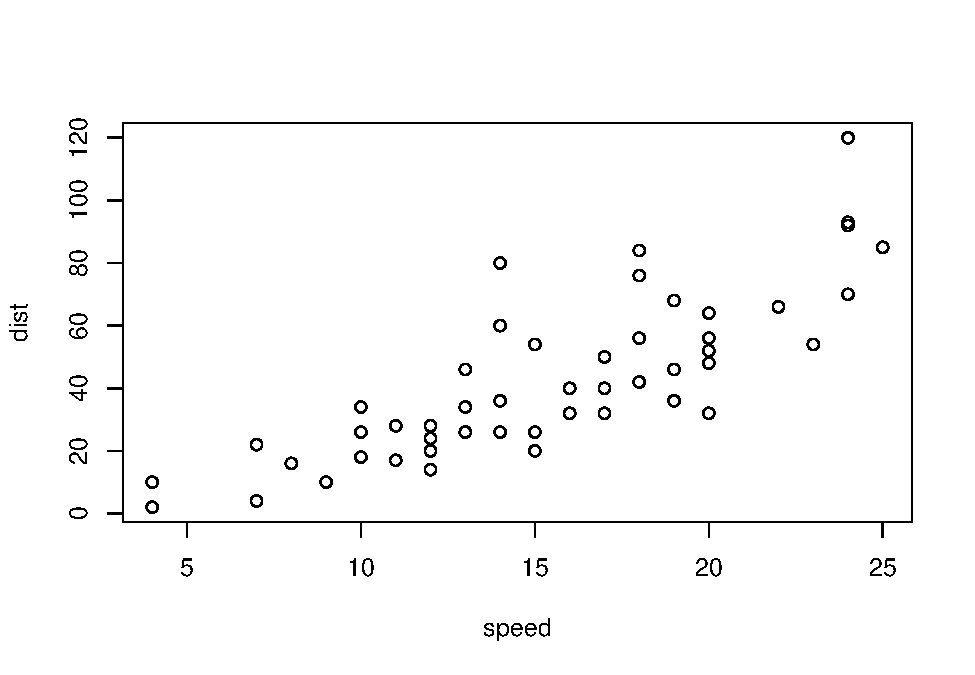
\includegraphics{Master-Thesis_files/figure-latex/plotCars-1.pdf}
\caption{\label{fig:plotCars}A car plot}
\end{figure}

\begin{Shaded}
\begin{Highlighting}[]
\CommentTok{# knitr::include_graphics(rep('_bookdown_files/Master-Thesis_files/fig1.png', 3))}
\end{Highlighting}
\end{Shaded}

\hypertarget{literature}{%
\chapter{Literature}\label{literature}}

Here is a review of existing methods.

\hypertarget{methods}{%
\chapter{Methods}\label{methods}}

We describe our methods in this chapter.

\hypertarget{applications}{%
\chapter{Applications}\label{applications}}

Some \emph{significant} applications are demonstrated in this chapter.

\hypertarget{example-one}{%
\section{Example one}\label{example-one}}

\hypertarget{example-two}{%
\section{Example two}\label{example-two}}

\hypertarget{final-words}{%
\chapter{Final Words}\label{final-words}}

We have finished a nice book.

\citet{Reid} \{Reid,
title = \{The origin of the 1918 pandemic influenza virus a
continuing enigma.\},
author = \{REID, A. H.\},
note = \{The Journal of General Virology\},
url = \{\url{https://yihui.org/knitr/}\},
year = \{2003\},
\}

\bibliography{book.bib,packages.bib}

\end{document}
